%  LaTeX support: latex@mdpi.com 
%  For support, please attach all files needed for compiling as well as the log file, and specify your operating system, LaTeX version, and LaTeX editor.

%=================================================================
\documentclass[algorithms,article,submit,pdftex,moreauthors]{Definitions/mdpi} 
%\documentclass[preprints,article,submit,pdftex,moreauthors]{Definitions/mdpi} 
% For posting an early version of this manuscript as a preprint, you may use "preprints" as the journal. Changing "submit" to "accept" before posting will remove line numbers.

%--------------------
% Class Options:
%--------------------
%----------
% journal: algorithms
%----------

%---------
% article
%---------
% The default type of manuscript is "article"

%----------
% submit
%----------
% The class option "submit" will be changed to "accept" by the Editorial Office when the paper is accepted. 

%------------------
% moreauthors
%------------------
% If there is only one author the class option oneauthor should be used. Otherwise use the class option moreauthors.

%---------
% pdftex
%---------
% The option pdftex is for use with pdfLaTeX. Remove "pdftex" for (1) compiling with LaTeX & dvi2pdf (if eps figures are used) or for (2) compiling with XeLaTeX.

%=================================================================
% MDPI internal commands - do not modify
\firstpage{1} 
\makeatletter 
\setcounter{page}{\@firstpage} 
\makeatother
\pubvolume{1}
\issuenum{1}
\articlenumber{0}
\pubyear{2025}
\copyrightyear{2025}
\datereceived{ } 
\daterevised{ } % Comment out if no revised date
\dateaccepted{ } 
\datepublished{ } 
%\datecorrected{} % For corrected papers: "Corrected: XXX" date in the original paper.
%\dateretracted{} % For retracted papers: "Retracted: XXX" date in the original paper.
\hreflink{https://doi.org/} % If needed use \linebreak
%\doinum{}
%\pdfoutput=1 % Uncommented for upload to arXiv.org
%\CorrStatement{yes}  % For updates

%=================================================================
% Add packages and commands here. The following packages are loaded in our class file: fontenc, inputenc, calc, indentfirst, fancyhdr, graphicx, epstopdf, lastpage, ifthen, float, amsmath, amssymb, lineno, setspace, enumitem, mathpazo, booktabs, titlesec, etoolbox, tabto, xcolor, colortbl, soul, multirow, microtype, tikz, totcount, changepage, attrib, upgreek, array, tabularx, pbox, ragged2e, tocloft, marginnote, marginfix, enotez, amsthm, natbib, hyperref, cleveref, scrextend, url, geometry, newfloat, caption, draftwatermark, seqsplit
% cleveref: load \crefname definitions after \begin{document}
\usepackage[algo2e,linesnumbered,ruled]{algorithm2e} 
\usepackage{tabularx}       % automatic column width
\usepackage{mathtools}  
\usepackage{amsfonts}       % mathbb
\usepackage{xfrac}          % slanted fractions
\usepackage{bm}             % bold greeks 
\usepackage{setspace}       % for controlled interline
\usepackage{graphicx}
\usepackage{amsmath}        % multiline formulas
\usepackage{array}          % for better column control
\usepackage{xcolor}         % for coloring blocks of text
\usepackage{rotating} 		 % for rotating wide tables

\usepackage{tikz}
\usetikzlibrary{positioning,fit,arrows.meta,decorations.pathreplacing,calc}
\tikzset{
	block/.style={draw, rounded corners, thick, minimum width=3.2cm, minimum height=8mm, align=center, font=\sffamily},
	mha/.style={block, fill=blue!6},
	ff/.style={block, fill=green!6},
	addnorm/.style={rectangle, draw, minimum height=5mm, inner sep=2pt, font=\scriptsize},
	encbox/.style={draw, dashed, rounded corners, inner sep=6pt},
	arrow/.style={-{Stealth[length=2mm,width=2mm]}, thick},
	small/.style={font=\scriptsize}
}

\setlength{\headheight}{24.2pt}
\SetAlgoNlRelativeSize{0}
\DontPrintSemicolon

%=================================================================
% Please use the following mathematics environments: Theorem, Lemma, Corollary, Proposition, Characterization, Property, Problem, Example, ExamplesandDefinitions, Hypothesis, Remark, Definition, Notation, Assumption
%% For proofs, please use the proof environment (the amsthm package is loaded by the MDPI class).

%=================================================================
% Full title of the paper (Capitalized)
\Title{\textcolor{blue}{Deconstructing a Minimalist Transformer Architecture for Univariate Time Series Forecasting}}

% MDPI internal command: Title for citation in the left column
\TitleCitation{Deconstructing transformer-based time series forecasting}

% Author Orchid ID: enter ID or remove command
\newcommand{\orcidauthorA}{0000-0002-1220-1235} % Add \orcidA{} behind the author's name
%\newcommand{\orcidauthorB}{0000-0000-0000-000X} % Add \orcidB{} behind the author's name

% Authors, for the paper (add full first names)
\Author{Filippo Garagnani $^{1}$ and Vittorio Maniezzo\orcidA{} $^{2,}$*}

%\longauthorlist{yes}

% MDPI internal command: Authors, for metadata in PDF
\AuthorNames{Filippo Garagnani and Vittorio Maniezzo}

% If this is a ACS style journal (Except for the above Chicago and APA journals, all others are in the ACS format): 
% Lastname, F.; Lastname, F.; Lastname, F.
\isAPAStyle{%
       \AuthorCitation{Garagnani, F.\& Maniezzo, V.}
         }{%
        \isChicagoStyle{%
        \AuthorCitation{Lastname, Firstname, Firstname Lastname, and Firstname Lastname.}
        }{
        \AuthorCitation{Garagnani, F.; Maniezzo, V.}
        }
}

% Affiliations / Addresses (Add [1] after \address if there is only one affiliation.)
\address{%
$^{1}$ \quad University of Modena and Reggio Emilia; 298707@studenti.unimore.it\\
$^{2}$ \quad Department of Computer Science, University of Bologna; vittorio.maniezzo@unibo.it}

% Contact information of the corresponding author
\corres{Correspondence: vittorio.maniezzo@unibo.it;}
%\secondnote{These authors contributed equally to this work.}
%\simplesumm{} % Simple summary

% Abstract (Do not insert blank lines, i.e. \\) 
\abstract{\textcolor{blue}{This paper provides a detailed breakdown of a minimalist, fundamental Transformer-based architecture for forecasting univariate time series. It describes each processing step in detail, from input embedding and positional encoding to self-attention mechanisms and output projection. All of these steps are specifically tailored to sequential temporal data. By isolating and analysing the role of each component, the paper demonstrates how Transformers capture long-term dependencies in time series. A simplified, interpretable Transformer model is implemented and showcased using a simple example, before being validated using a significant benchmark suite. This suite includes datasets from forecasting competitions and real-world applications. The aim of this work is to serve as a practical guide and foundation for future transformer-based forecasting innovations.}}

% Keywords
\keyword{Data series forecasting; Transformer models; Machine learning} 

\begin{document}
%%%%%%%%%%%%%%%%%%%%%%%%%%%%%%%%%%%%%%%%%%
\section{Introduction} \label{sec:intro}

Time series forecasting is a key topic in data science and has a wide range of applications in areas such as economics, energy, healthcare, logistics and environmental monitoring. Accurate forecasting enables informed decision-making, efficient resource allocation and risk mitigation. Traditional statistical methods such as ARIMA and exponential smoothing have long been used for this purpose and often produce good results when the necessary assumptions are met. However, these methods often struggle to capture complex patterns and long-term dependencies in the data, an area in which deep learning methods, especially sequence models such as recurrent neural networks (RNNs), have often demonstrated superior performance.

Transformer models, which were initially designed for natural language processing tasks, have recently shown remarkable success in understanding and generating sequential data, demonstrating their effectiveness in modelling long-range dependencies. Transformers are attention-based models that eliminate the need for recurrence and convolution, relying instead on a self-attention mechanism to capture global context across sequences. This architecture has had a revolutionary impact on NLP, and its application to time series forecasting is a rapidly growing area of research. 

Unlike natural language, time series are composed of continuous values and frequently exhibit seasonality, trends and influence from exogenous variables. While recent studies have proposed various adaptations of the transformer to address the unique properties of time series data, many of these models are treated as opaque black boxes. This means that there is limited clear understanding of how each component relates to temporal information and contributes to forecasting performance. Furthermore, the implementation details are frequently insufficiently specified, which makes reproducibility and interpretability challenging.

In this paper, our aim is to 'deconstruct' the forecasting process of transformer-based models when applied to univariate time series. Our objective is to provide a transparent, modular and pedagogical account of how univariate time series are transformed and processed within these models to generate future trajectories. Each processing step is described in detail, including data normalization, input windowing, positional encoding, encoder and decoder architecture, training strategies, and prediction generation. Both the theoretical basis and the practical design choices are highlighted, showing how each element contributes to predictive accuracy and attempting to bridge the gap between theoretical advancements and practical implementation.

To validate our methodology, a basic transformer-based model has been implemented and evaluated on a significant benchmark of univariate time series. These were selected from the well-known M forecasting competition benchmarks and included macro- and micro-economic, industrial, financial and demographic series with varying statistical properties. The work combines theoretical explanation with empirical validation to serve as a comprehensive guide to deconstructing transformer-based time series forecasting, providing a tutorial for newcomers and a reference for practitioners.

The paper is structured as follows. Section \ref{sec:literature} reviews the related works in time series forecasting, with particular emphasis on recent advancements leveraging Transformer architectures. Section \ref{sec:transformer} presents the workflow of a minimalist Transformer module to produce a multipoint forecast for a univariate time series. Section \ref{sec:results} analyses some results in applying the described architecture on benchmark data series and comparing it with another standard methodology.

%%%%%%%%%%%%%%%%%%%%%%%%%%%%%%%%%%%%%%%%%%
\section{Related work} \label{sec:literature}

Transformer modules for processing graph-like structures were originally introduced in \citep{LBB97} for a check-reading task, however it was only with \citep{VSPU17} that the current transformer architecture for sequence modelling was proposed. Already the very first line of the introduction of this seminal paper frames the transformer architecture among established time series modelling and forecasting algorithms, citing LSTM \citep{HS97} and GRU \citep{ CGCB14}, i.e., the two main architectures for recurrent neural networks (RNN) applied to time series modelling.

Indeed, RNNs can be effective in capturing long-term dependencies among data, but suffer from slow training, vanishing gradients and high sensitivity to hyperparameter settings. Furthermore, the most well-established statistical methods, such as autoregressive integrated moving average (ARIMA) \citep{BJ70} and exponential smoothing (ETS) \citep{H57,W60}, are highly effective for stationary data but struggle with complex nonlinear patterns.

\textcolor{blue}{Transformer architectures are immune to these drawbacks because they do not rely on the assumption of stationarity. They capture global dependencies in input sequences without relying on recurrence, instead leveraging self-attention mechanisms to enable the direct modelling of long-range dependencies. This supports full parallelization during training and allows the model to focus on relevant time steps, regardless of their position in the sequence}.

A key challenge in applying transformers to univariate time series is the absence of the rich semantic tokens found in language. Unlike words in a sentence, time series values are continuous and lack discrete meaning, making it more difficult to learn meaningful attention patterns. Therefore, transformers need to be adapted for time series forecasting. Early adaptations of transformers for use with time series data include:

\begin{description}
	\item Informer \citep{ZZPZ21}, which introduces a sparse self-attention mechanism to reduce the quadratic complexity of self-attention, making it more efficient for long sequence time series forecasting.

	\item Autoformer \citep{WXWL22}, which integrates a series decomposition block within the transformer to separate trend and seasonal components obtaining a decomposition-based attention for better seasonal-trend modeling, improving interpretability and long-horizon forecasting accuracy.

	\item FEDformer \citep{ZMWW22}, which incorporates Fourier transformations into the attention mechanism to better exploit frequency-domain characteristics.

	\item PatchTST \citep{patchTST}, which employs a splitting mechanism to time series, converting multiple timesteps (i.e., a patch) into a single token, enabling a vanilla Transformer architecture to capture long-term dependencies with fewer tokens. 
\end{description}

More recently, an explosion of adaptations has appeared, together with dedicated surveys and tutorials \cite{ WZZC23, ANTS23, SZLW25}. However, these models are often complex, incorporating multiple components such as static covariates, gating mechanisms, and probabilistic outputs. While these additions have shown empirical gains, they frequently obscure the core dynamics of the attention mechanism and make the models less accessible for analysis or adaptation.

By contrast, there is interest in minimal Transformer implementations, which isolate the effectiveness of self-attention in forecasting tasks. Informer has already demonstrated that a simplified Transformer, devoid of specialized components, can outperform classical models and RNNs on certain benchmarks when properly tuned. Similarly, \citep{LSNP21} proposed the `Temporal Attention' module within a lightweight Transformer framework, demonstrating that attention over timesteps alone can achieve comparable performance on univariate series. Other studies, such as iTransformer \cite{LHZW24}, investigate how the performance of standard Transformers is affected by different initialization, normalization, or positional encoding strategies. This sheds light on the contribution of each component to forecasting accuracy.

This body of work highlights the growing interest in demystifying transformer-based time series models by removing layers of abstraction. In line with this perspective, a minimalist transformer specifically designed for univariate forecasting is proposed. A minimal version of the transformer encoder has been developed by maintaining only the essential self-attention and feedforward components. By simplifying the model, our aim is to understand the fundamental processes that enable transformers to succeed in this domain and to provide a transparent and reproducible basis for further research.

% https://medium.com/intel-tech/how-to-apply-transformers-to-time-series-models-spacetimeformer-e452f2825d2e

%%%%%%%%%%%%%%%%%%%%%%%%%%%%%%%%%%%%%%%%%%
\section{The transformer processing pipeline} \label{sec:transformer}

This section describes the successive processing phases carried out by a minimalist transformer module to produce a multipoint forecast of a univariate data series. The relevant python code can be found in \cite{G25}. Successive processing stages are here showcased on a tiny time series obtained by querying Google Trends \cite{googletrends2025} on the term "restaurant". The series shows a trend (at the time of writing, it is holiday season in Italy and interest in dining out is increasing) as well as seasonality, due to increased interest at weekends. Only 35 data points are considered, 7 of which are kept for validation and 28 are used for training.

The series $s(t)$ is the following:
\begin{align}
s(t) = (& 44, 48, 51, 48, 50, 63, 66, 48, 53, 56, 52, 57, 70, 67, 56, 60, 62, 60, 58, 75, 73, 59, 61, 65,\nonumber\\
        & 63, 63, 78, 80, 63, 64, 67, 65, 70, 87, 84)\nonumber
\end{align}

The data processing cycle consists of three main phases: encoding, decoding, and learning. A view of the whole model can be seen in Figure \ref{fig:trans}. The following subsections provide details on each phase, the reader is referred to \cite{VSPU17} for a more exhaustive exposition.

\begin{figure}
	\centering
	\begin{tikzpicture}[node distance=10mm, minimum width=22mm]
		
		% Encoder stack
		\node (encin) [block, fill=gray!10] {Source Input Embeddings};
		\node (enc) [block, fill=blue!10, below=of encin, minimum height=30mm] {Encoder \\ $\times n$};
		\node (encout) [block, fill=gray!10, below=of enc] {Encoder Output};
		
		% Decoder stack
		\node (decin) [block, fill=gray!10, right=20mm of encin] {Target Input Embeddings};
		\node (dec) [block, fill=green!10, below=of decin, minimum height=40mm] {Decoder \\ $\times l$};
		\node (decout) [block, fill=gray!10, below=of dec] {Decoder Output};
		
		% Arrows for Encoder
		\draw[arrow] (encin) -- (enc);
		\draw[arrow] (enc) -- (encout);
		
		% Arrows for Decoder
		\draw[arrow] (decin) -- (dec);
		\draw[arrow] (dec) -- (decout);
		
		% Cross connection: encoder output into decoder
		\draw[arrow] (encout.east) -- ++(15mm,0) |- (dec.west);
		\draw[dashed,->] (decout.east) -- ++(10mm,0) |- (decin.east)
			node[pos=0.25,right] {\scriptsize Autoregressive};
		
		% Labels
		\node[above=0mm of encin.north] {\textbf{Encoder Side}};
		\node[above=0mm of decin.north] {\textbf{Decoder Side}};
		
	\end{tikzpicture}
	\caption{The vanilla Transformer architecture.}
	\label{fig:transformer}
\end{figure}


\subsection{Encoding} \label{subsec:encoding}

The objective of the encoding component (i.e., the \textit{encoder}) in a Transformer architecture is to process an input sequence and convert the raw input into a contextually enriched representation that captures both local and global dependencies. This representation can then be used effectively by the rest of the model.

\begin{figure}
	\centering
	\begin{tikzpicture}[node distance=6mm]
	
	\node (input) [block, fill=gray!10] {Input embeddings \\ \scriptsize (8)};
	\node (pe) [block, fill=gray!10, below=of input] {+ Positional Encoding \\ \scriptsize (28)};
	
	
	\node (mha) [mha, below=of pe] {Multi-Head Attention \\ \scriptsize (80)};
	\node (add1) [addnorm, below=of mha] {Add \& Norm 1 \par \scriptsize (8)};
	
	% Feedforward
	\node (ff) [ff, below=of add1] {Feedforward Network \\ \scriptsize (148)};
	\node (add2) [addnorm, below=of ff] {Add \& Norm 2 \par \scriptsize (8)};
	
	% Output
	\node (output) [block, fill=gray!10, below=of add2] {Output};
	
	% Arrows
	\draw[arrow] (input) -- (pe);
	\draw[arrow] (pe) -- (mha);
	\draw[arrow] (mha) -- (add1);
	\draw[arrow] (add1) -- (ff);
	\draw[arrow] (ff) -- (add2);
	\draw[arrow] (add2) -- (output);
	
	% Box around the encoder block
	\node[draw, dashed, rounded corners, fit=(mha) (add2), inner sep=6pt] (encbox) {};
	\node[right=2mm of encbox.east] (enclabel) {Encoder Block};
	\node[below=0mm of enclabel.south] {$\times n$};
	
	\end{tikzpicture}
	\caption{The Encoding Process. For each block, the total number of learnable parameters for the restaurant series example is shown.}
	\label{fig:enc}
\end{figure}

The general structure of the encoding module is represented by the pseudocode in Algorithm \ref{algo:encoding} and sketched in Figure \ref{fig:enc}. All intermediate numerical results obtained for the restaurant series case study are reported in appendix \ref{sec:appendix} to enable the interested reader to immediately grasp the dimensionalities and values involved in this tiny example, and possibly to follow the corresponding evolution of a run of the code provided in \cite{G25}. In the case of the running example the following argument values are used: $n$=7, $m$=4, $k$=2, $d_k$=$d_v$=2, $p$=16.

The individual steps are detailed below.

\begin{algorithm2e}
	\SetKwInOut{Input}{Input}
	\SetKwInOut{Output}{Output}
	\SetKw{KwGoTo}{go to}

	\underline{procedure encoding(s,n,m,k,$d_k$,$d_v$,$p$)} \label{algo:encoding}
	
	\Input{ A time series ${\bf s} = [s_i]$, $i=0,\,\ldots,\,t$}
	\Output{ A 2D matrix $Z$}
	
	\tcp*{Input Projection}
	\tcp*{transform the array {\bf s} into the 2D embedding matrix (tensor) {\bf X}} 
	\For{i = 0, \ldots, t} 
	{\label{enc:seca1}
	   Expand value $s_i$ into a row $X_i = (s_iW_i) + b_i$
	}   \label{enc:seca2}
	
	X' = X + P; \tcp*{Positional encoding} \label{enc:positional}
        
	\For{n times}
	{ \label{enc:encoding-block1}
            \tcp*{multihead attention}
            \For{h = 1, \dots, k}
            {	\label{enc:multihead1}
                \tcp{attention}
                Compute $Q^h=(X'\cdot W_q^h) + b_q^h$;\; \label{enc:qh}
                Compute $K^h=(X'\cdot W_k^h) + b_k^h$;\; \label{enc:kh}
                Compute $V^h=(X'\cdot W_v^h) + b_v^h$;\; \label{enc:vh}
                Let $d_k=$ num columns of $W^h_k$;\; \label{enc:dk}
                Let $A^h = \dfrac{Q \cdot K^T}{\sqrt{d_k}}$; \tcp*{init attention function} \label{enc:attention1}
                Let $A^h = softmax\left(A^h\right)$; \tcp*{softmax over all rows} \label{enc:softmax}
                Let $A^h = A^h\cdot V^h$; \tcp*{completed attention function} \label{enc:attention2}
            } \label{enc:multihead2}
            Let $A=concatenate(A^h)$, $h=0,\dots,k$;\; \label{enc:concatenation}
            Let $A = A \cdot W_O$; \tcp*{output projection} \label{enc:outproj} 
            Let $X' = LayerNorm(X' + A)$;\; \label{enc:addnorm1}
            Let $F = feedforward(X')$; \tcp*{feedforward layer} \label{enc:ffn}
            Let $X' = LayerNorm(X' + F)$;\; \label{enc:addnorm2}
        }   \label{enc:encoding-block2}                  
        Let $Z = X'$; \label{enc:output}
	\caption{The encoding module}
\end{algorithm2e}

~\\(\textit{Input arguments})

The input consists of the data series to be forecast, in our case, it is an array $s \in \mathbb{R}^n$ and of six control hyperparameters.

For the restaurant time series, a straightforward preprocessing step has been applied: \textit{min-max} normalization of the raw data. Subsequently, each sequence was constructed using a sliding window of length $n = 7$ over the series.

~\\Lines \ref{enc:seca1}-\ref{enc:seca2}: (\textit{Input Projection})

Single scalar values for each single timestep may not be expressive enough to capture contextual information. Each data point is projected into a higher-dimensional space where nonlinear dependencies between features can be easier to identify. 

In our minimalist transformer model the projections, also known as {\em embeddings}, were obtained by multiplying each datapoint by a shared real-valued vector $W_i \in \mathbb{R}^m$ initialized as a random gaussian vector, and by adding a bias array $b_i \in \mathbb{R}^m$. These values can later be learned. In this way, a matrix $X \in \mathbb{R}^{n\times m}$ is computed, which contains, for each original timestep, its $m$-dimensional representation.

In the restaurant series, the projections were based on vectors of 4 values, obtaining a set of matrices, each of which with $n=7$ rows and $m=4$ columns, leaving $4$ parameters to be learned for the projection vector, and other $4$ for the bias array. Each matrix {\bf X} represents a window over the input time series, the first of these matrices is presented in the appendix as table \ref{tab:matX}. The learned arrays $W_i, b_i$ are also shown in the appendix, as table \ref{tab:seca}.

~\\Line \ref{enc:positional}: (\textit{Positional Encoding})

The basic attention mechanism, which will be implemented in lines \ref{enc:attention1}-\ref{enc:attention2}, is insensitive to the permutation of the input values \cite{VSPU17} and is in itself unusable for modelling data series. Therefore, the model does not inherently deal with the sequential position of the elements: the attention only depends on the set of elements, not on their order. To inject ordering information, each input embedding $X^j$ is added to a positional vector. 
This is obtained by means of a matrix $P \in \mathbb{R}^{n \times m}$, which yields the transformed input: 
\begin{equation}
    X' = X + P
\end{equation}
where $n$ denotes the sequence length and $m$ the embedded dimension.

The matrix $P$ can be either \textit{static}, remaining fixed during the training phase, or \textit{learnable}, changing at each step to better adapt to the task at hand. It can also be either \textit{absolute}, depending solely on the element's position, or \textit{relative}, in which case the element itself influences the values of the matrix's rows. 

In the proposed minimalist architecture, matrix $P \in \mathbb{R}^{7 \times 4}$ is an absolute, learnable positional encoding, in the restaurant use case consisting of 7 rows and 4 columns. This equates to further 28 parameters that need to be learned. The matrix $P$ used in our running example is presented in the appendix as table \ref{tab:matP}. 

~\\Lines \ref{enc:encoding-block1}-\ref{enc:encoding-block2}: (\textit{Encoding Blocks})

The main loop of the algorithm repeats $n$ times a block of code called an {\it Encoding Block}. In it, matrix {\bf X} is first passed to a module implementing Multihead Attention (Lines \ref{enc:multihead1}-\ref{enc:multihead2}). The outputs of the heads are then concatenated and projected to keep the size consistent (Lines \ref{enc:concatenation}-\ref{enc:outproj}). Next, a residual connection with a normalization is applied (Line \ref{enc:addnorm1}). The output is then passed through a small feedforward network after which another residual connection and normalization are applied (Lines \ref{enc:ffn}-\ref{enc:addnorm2}).
It's important to note that each iteration uses its own set of parameters for the projections, attention weights, and feedforward layers; parameters are not shared between iterations.
All these steps are detailed in the following.

~\\Lines \ref{enc:multihead1}-\ref{enc:multihead2}: (\textit{Multihead Attention})

This loop iterates a basic attention mechanism that dynamically weighs the contribution of each past point in the series when computing the representation of those under scrutiny. It computes a set of attention scores relating the "query" vector of the current point and "key" vectors of all sequence values. \#In our application, a query comes from the embedding of the last known observation while the keys correspond to those of all past observations.\# The resulting attention weights determine which points matter most and the forecast is then given by a weighted sum of the corresponding "value" vectors.

Queries (the elements currently focused on), keys (descriptors of the corresponding values), and values (the actual information) are all represented as matrices. Typically, queries and keys share the same inner dimension $d_k$, while values may have a different dimension $d_v$. At each iteration the corresponding set of query, key, and value is referred to as a \textit{head}. The matrices and the bias identified for the two heads used in our running example are reported in the appendix in tables \ref{tab:matWq} and \ref{tab:bias} .

~\\Line \ref{enc:qh}: generates the $h-th$ query matrix and projects the input embeddings into vectors that represent what it has been looked for in the past. This is achieved by using a dynamic parameter matrix $W^h_q \in \mathbb{R}^{m \times d_k}$ and a bias array $b^h_q \in \mathbb{R}^{d_k}$ that are learnt.

~\\Line \ref{enc:kh}: generates the $h-th$ key matrix and projects the input embeddings into vectors that represent the information content of each corresponding embedding. This is achieved by using a dynamic parameter matrix $W^h_k \in \mathbb{R}^{m \times d_k}$ and a bias array $b^h_k \in \mathbb{R}^{d_k}$ that are learnt.

~\\Line \ref{enc:vh}: generates the $h-th$ value matrix and projects the input embeddings into vectors that represent the relevant information of each available embedding. This is achieved by using a dynamic parameter matrix $W^h_v \in \mathbb{R}^{m \times d_v}$ and a bias array $b^h_v \in \mathbb{R}^{d_k}$ that are learnt.

~\\Line \ref{enc:dk}: initializes the scaling factor.

~\\Line \ref{enc:attention1}: implements the first part of the attention function, in this case using the \textit{Scaled Dot-Product Attention} \cite{VSPU17}. The similarity between sequence elements is computed from $Q$ and $K$ through a dot product. The key matrix is transposed so that the operation compares each feature of every query with the corresponding feature of every key. This initial $A$ matrix will contain similarity values $a_{ij} \in \mathbb{R}$ between every query vector and every key vector. 

~\\Line \ref{enc:softmax}: transforms the similarity values into `probability' scores. The $\text{softmax}()$ operator is applied to all elements $a_{ij}$ over every row: $a_{ij} = e^{a_{ij}} / \sum_k e^{a_{kj}},\quad \forall i,j  = 1,\,...,\,n $. In this way, for every query vector, normalized weights of similarity towards key vectors are obtained. 

~\\Line \ref{enc:attention2}: completes the computation of the attention function by implementing a weighted sum of the value vectors, $A^h = A^h \cdot V^h$, thereby aggregating information from the relevant timesteps.

~\\Line \ref{enc:concatenation}: lines \ref{enc:multihead1}-\ref{enc:multihead2} are repeated $k$ times, each time obtaining an attention matrix $A^h$, $h=1,\dots,k$. This line concatenates all these matrices in a single bigger one, $A = [A^1\;A^2\;...\;A^h]$. The matrix $A$ obtained for the running example is reported in the appendix as table \ref{tab:matA}.

~\\Line \ref{enc:outproj}: since concatenation may modify the dimensionality, a final output projection $W^O \in \mathbb{R}^{hd_v \times m}$ is applied to ensure that the original size is kept $X' = A \cdot W^O$. 

~\\In our architecture, we set $h = d_k = d_v = \frac{m}{2} = 2$. This produced six matrices, all of size $4 \times 2$, totaling $48$ more parameters to learn. The output matrix $W^O$ is, instead, of size $4 \times 4$. Matrix $W^O$ for the running example is reported in table \ref{tab:matWO} of the appendix.

~\\Lines \ref{enc:addnorm1}, \ref{enc:addnorm2}: (\textit{Add \& Norm})

This block tries to stabilize training by normalizing activations while keeping a residual path. It is implemented by a layer function $LayerNorm : \mathbb{R}^{n \times m} \to \mathbb{R}^{n \times m}$, that operates independently for each row $i$ (i.e., for each embedding), computing the mean $\mu_i \in \mathbb{R}$ and the variance $\sigma_i \in \mathbb{R}$, and updating the features of row $i$ as $ x_{ij} = \gamma_j\cdot\dfrac{x_{ij} - \mu_i}{\sigma_i} + \beta_j$, 
where $\gamma,\beta \in \mathbb{R}^m$ are learnable parameters.

In our minimalist architecture, having set $m = 4$, and having two different \textit{LayerNorm} blocks, $16$ parameters were set to be learned. For the first layer:
$$
    \gamma =    \begin{bmatrix}
                    0.8659 & 1.1768 & 0.4843 & 1.2575
                \end{bmatrix} \quad
    \beta =     \begin{bmatrix}
                -0.3721 & 0.1294 & -0.0496 & 0.3132
                \end{bmatrix}
$$
While for the second layer:
$$
    \gamma =    \begin{bmatrix}
                    0.8747 & 0.7511 & 0.6320 & 0.7074
                \end{bmatrix} \quad
    \beta =     \begin{bmatrix}
                    -0.1117 & -0.1993 & 0.0806 & 0.1641
                \end{bmatrix}
$$

~\\Line \ref{enc:ffn}: (\textit{Feedforward Network})

The final processing step of our minimalist transformer architecture implements a two-layer network, with a ReLU activation function in between:
\begin{equation}
    s' \leftarrow \text{max}(0,\,s'\cdot W_1 + b_1) \cdot W_2 + b_2
\tag{Line \ref{enc:ffn}}
\end{equation}
where:
$$
    W_1 \in \mathbb{R}^{m \times p},\quad
    b_1 \in \mathbb{R}^{p}
$$ $$
    W_2 \in \mathbb{R}^{p \times m},\quad
    b_2 \in \mathbb{R}^m
$$

The ReLU function is applied element-wise. The intermediate dimension $p$ is typically chosen larger than $m$ to improve model capacity and generalization. 

In our model, we set $p = 4 \times m = 16$, meaning a total number of $16 \times 4 \times 2 + (16 + 4) = 148$ parameters, as resulting also in Figure \ref{fig:enc}.
The values learned by the sample architecture is reported in the appendix in tables \ref{tab:matW1b1} and \ref{tab:matW2b2}.

~\\Line \ref{enc:output}: (\textit{Output})

The full output, stored in the matrix $X'$, contains the \textit{encoded} representation of the input timesteps. In order to distinguish it thereafter it will be denoted as $Z$. 

\subsection{Decoding} \label{subsec:decoding}

The objective of the decoding component (i.e., the decoder) in a transformer architecture is to generate an output sequence step by step. This is achieved by using the encoded representation of the input and the output data generated by the encoding component.

The general structure of the decoding module is represented by the pseudocode in Algorithm \ref{algo:decoding} and in Figure \ref{fig:dec}. The individual steps are detailed below.

\begin{figure}
    \centering
    \begin{tikzpicture}[node distance=6mm]
    
    % Input Embeddings + Positional Encoding
    \node (input) [block, fill=gray!10] {Input embeddings \\ \scriptsize (8)};
    \node (pe) [block, fill=gray!10, below=of input] {+ Positional Encoding \\ \scriptsize (28)};
    
    % Masked MHA
    \node (mha1) [mha, below=of pe] {Masked Multi-Head Attention \\ \scriptsize (80)};
    \node (add1) [addnorm, below=of mha1] {Add \& Norm \par \scriptsize (8)};
    
    % Encoder-Decoder MHA
    \node (mha2) [mha, below=of add1] {Multi-Head Cross-Attention \\ \scriptsize (80)};
    \node (add2) [addnorm, below=of mha2] {Add \& Norm \par \scriptsize (8)};
    
    % Feedforward
    \node (ff) [ff, below=of add2] {Feedforward Network \\ \scriptsize (148)};
    \node (add3) [addnorm, below=of ff] {Add \& Norm \par \scriptsize (8)};
    
    % Output
    \node (output) [block, fill=gray!10, below=of add3] {Output};
    
    % Arrows
    \draw[arrow] (input) -- (pe);
    \draw[arrow] (pe) -- (mha1);
    \draw[arrow] (mha1) -- (add1);
    \draw[arrow] (add1) -- (mha2);
    \draw[arrow] (mha2) -- (add2);
    \draw[arrow] (add2) -- (ff);
    \draw[arrow] (ff) -- (add3);
    \draw[arrow] (add3) -- (output);
    
    % Box around the decoder block
    \node[draw, dashed, rounded corners, fit=(mha1) (add3), inner sep=6pt] (decbox) {};
    \node[right=2mm of decbox.east] (declabel) {Decoder Block};
    \node[below=0mm of declabel.south] {$\times l$};
    
    % Extra arrow from Encoder output to second MHA
    \node (encout) [left=10mm of mha2] {Encoder Output $\textbf{Z}$};
    \draw[arrow] (encout) -- (mha2.west);
    
    \end{tikzpicture}
    \caption{The Decoding Process. For each block, the total number of learnable parameters for the restaurant series example is shown.}
    \label{fig:dec}
\end{figure}


\begin{algorithm2e} 
	\SetKwInOut{Input}{Input}
	\SetKwInOut{Output}{Output}
	\SetKw{KwGoTo}{go to}

        \underline{procedure decoding({\bf Z},no,l,$h^1$,$h^2$)} 
        
        \Input{ Matrix {\bf Z} from encoding, $no$ num data series points in output, $l$ number of decoding blocks, $h^1$ and $h^2$ head numbers} 
        \Output{ A 2D matrix ${\bf Y}$}
        
        \tcp*{subscripts indicate rows, superscripts columns}
        \label{dec:start}
        $\textbf{Y} = \textbf{0}_{no + 1 \times m}$ \; 	\label{dec:output}
        Let $Y^0 = \texttt{<CLS>}$ \;					\label{dec:cls}
        \For{i = 0, \ldots, no} 
	{       \label{dec:outer}
            \For{l times}
            {	\label{dec:decblock1}
                \tcp*{Masked self-attention}
                \For{j = 0, \dots, $h^1$}
                {   \label{dec:self1}
                    Let $Q^j$ = $(\textbf{Y}W_{q1}^j) + b_{q1}^j$,  \,\, 
                            $K^j$ = $(\textbf{Y}W_{k1}^j) + b_{k1}^j$,  \,\, 
                            $V^j$ = $(\textbf{Y}W_{v1}^j) + b_{v1}^j$   \;
                            \label{dec:selfproj}
                    Let $S^j = \dfrac{Q^j{K^j}^T}{\sqrt{d_k}}$\; \label{dec:scaled1}
                    Set $S_i^j=-\infty$ for all $i>j$; \tcp*{mask future positions}
                    \label{dec:masking}
                    Let $A^j = softmax\left(S^j\right)V^j$
                    \label{dec:softmax}
                }   \label{dec:self2}
                Let $\textbf{A}=concatenate(A^j)$, $j=0,\dots,h^1$\; \label{dec:concatenation1}
                Let {\bf A} = ${\bf A \cdot W_{o1}}$; \tcp*{for dimensionality coherence} \label{dec:outproject1}
                Let $\textbf{Y} = LayerNorm(\textbf{Y} + \textbf{A})$\; \label{dec:norm1}
                \tcp*{Cross-attention}
                \For{j = 0, \dots, $h^2$}
                {   \label{dec:cross1}
                    Let $Q^j=(\textbf{Y}\cdot W_{q2}^j) + b_{q2}^j$, \,\,
                            $K^j=(\textbf{Z}\cdot W_{k2}^j) + b_{k2}^j$, \,\, 
                            $V^j=(\textbf{Z}\cdot W_{v2}^j) + b_{v2}^j$\;
                    \label{dec:crossproj}
                    Let $A^{j} = softmax\left(\dfrac{Q^j{K^j}^T}{\sqrt{d_k}}\right)V^j$\;
                    \label{dec:scaled2}
                }   \label{dec:cross2}
                Let $\textbf{A}=concatenate(A^j)$, $j=0,\dots,h^2$\;
                \label{dec:concatenation2}
                Let {\bf A} = ${\bf A \cdot W_{o2}}$\;
                \label{dec:outproject2}
                Let $\textbf{Y} = LayerNorm(\textbf{Y} + \textbf{A})$\;
                \label{dec:norm2}
                Let $F = feedforward({\bf Y})$\;
                \label{dec:ffn}
                Let $\textbf{Y} = LayerNorm(\textbf{Y} + F)$\;
                \label{dec:norm3}
            } \label{dec:decblock2}
            $Y^{i + 1} = feedforward(Y^{i + 1})  * scale(\textbf{Z}) + bias(\textbf{Z})$\; \label{dec:finalproj}
            $y_i$ = ($Y^{i + 1}$)$W_o + b_o$
        } \label{dec:outer2}                     
    	\caption{The decoding module} 
    \label{algo:decoding}
\end{algorithm2e}

~\\Lines \ref{dec:start}-\ref{dec:output}: (\textit{Input})

The Decoder takes the encoder output $Z \in \mathbb{R}^{n \times m}$ as its main input (Line \ref{dec:start}) and iteratively updates a sequence represented by matrix $\textbf{Y} \in \mathbb{R}^{no + 1 \times m}$, where each row $Y_{i+1}$ represents the $i$-th output embedding, except for the first row which has a special row. Initially, the matrix is zero-initialized (Line \ref{dec:output}). The first row is set as the \texttt{<CLS>} token (Line \ref{dec:cls}), a learnable embedding used in order to kick-start the learning process. The sequence is then updated autoregressively, i.e., one timestep at a time with each new element depending on the previously generated ones.

The learned \texttt{<CLS>} token for the restaurant series is the following vector:
$$
	\texttt{<CLS>} = 	\begin{bmatrix}
		0.3162 & -0.1322 & 0.3443 & 0.2043
						\end{bmatrix}
$$

~\\Lines \ref{dec:decblock1}-\ref{dec:decblock2}: (\textit{Decoding Blocks})

Just as in the encoding phase, the main loop of the algorithm updates for $l$ iterations (Lines \ref{dec:decblock1}–\ref{dec:decblock2}) the matrix $\textbf{Y}$. The block of code implementing each iteration is called a \textit{Decoding Block}.
In the block, matrix {\bf Y} is first processed by the {\em Multihead Masked Self-Attention} which enables the decoder to process to previous positions in the output sequence while preventing it from attending to future positions, thereby enforcing autoregressive generation.
Next, $\mathbf{Y}$ interacts with the encoder output $\mathbf{Z}$ through a {\em Multihead Cross-Attention module} which enables the model to selectively focus on relevant parts of the input sequence (as encoded by the encoder) when generating each output token. This is the key mechanism that connects the encoder and decoder.
Finally, the output is passed through some postprocessing steps to produce the final result of the single iteration.

%As above, every iteration has its own learnable parameters: the projection matrices, the attention weight matrices, and the feedforward layers are re–initialized independently for each step of the loop. No parameter sharing occurs across different iterations.
%In the employed architecture, we set $l = $. 

The general procedure outlined above is explained in more detail below.

~\\Lines \ref{dec:self1}-\ref{dec:outproject2}: (\textit{Masked Self-Attention})

The Masked Self-Attention mechanism works in the same way as a Multihead Attention function, but ensures that the generation of each successive sequence value can only consider the present or the past, never the future. This is achieved using a look-ahead mask that prevents feedback in time.
The following operations are performed inside each loop (i.e. each head).

~\\Line \ref{dec:selfproj}: generates the query, key and value matrices, projecting the already-generated embeddings into semantic vectors. This projection is achieved by using dynamic parameter matrices and a dynamic bias array, both of which must be learnt.

~\\Line \ref{dec:scaled1}: computes the first part of the \textit{Scaled-Dot Product Attention} function.

~\\Line \ref{dec:masking}: masks out any similarity values computed between a query vector from a timestep and a key vector coming from a future timestep. During the subsequent softmax step, the value $-\infty$ becomes 0, thus avoiding dependency on the future.

~\\Line \ref{dec:softmax}: computes the last part of the attention function.

~\\After the loop of Lines \ref{dec:selfproj}-\ref{dec:softmax} is completed, the $h^1$ different output matrices must be aggregated together.

~\\Line \ref{dec:concatenation1}: the $h^1$ matrices are concatenated by row, obtaining the complete \textbf{A} matrix.

~\\Line \ref{dec:outproject1}: the matrix \textbf{A} is multiplied by $W_{o1} \in \mathbb{R}^{h^1d_v \times m}$. The latter matrix is a learnable parameter.

~\\The operations above are referred to as 'Self-Attention' because the projections of $Q, K$ and $V$ all come from the same input vector, $\textbf{Y}$. In our example architecture, we set the number of heads for the self-attention layers to $h^1 = 2$.

~\\Lines \ref{dec:norm1}, \ref{dec:norm2}, \ref{dec:norm3}: (\textit{Add \& Norm})
Each operation in the decoding stage is followed by a residual connection and a normalization step. The $\text{LayerNorm}()$ function works row-wise on the embeddings, standardizing them with learnable scaling and shifting parameters ($\gamma, \beta$).

~\\Lines \ref{dec:cross1}-\ref{dec:outproject2}: (\textit{Cross-Attention})

\noindent The second Attention step in the decoding phase links the partially generated output with the encoder’s representation of the input. Specifically, the decoder’s current output is projected into queries, while the encoder’s output provides the keys and values. Similar to Multihead Attention, this process involves a loop (Lines \ref{dec:cross1}-\ref{dec:cross2}) and an aggregation step at the end (Lines \ref{dec:concatenation2}-\ref{dec:outproject2}).

~\\Line \ref{dec:crossproj}: generates the query, key, and value matrices, projecting the decoder’s current output into queries and the encoder’s output into keys and values. Each projection uses a learnable parameter matrix to transform the embeddings into semantic vectors.

~\\Line \ref{dec:scaled2}: computes the attention function, using the already computed matrices.

~\\The above operations are repeated $h^2$ times, getting $h^2$ attention outputs.

~\\Line \ref{dec:concatenation2}: All the head's outputs are concatenated by the rows in a single matrix $\textbf{A}$.

~\\Line \ref{dec:outproject2}: The attention matrix $\textbf{A}$ is multiplied by $W_{o2} \in \mathbb{R}^{h^2d_v \times m}$, which is a learnable parameter.

~\\The name Cross-Attention is due to the fact that the output of the encoding phase $Z$ and the decoding current output $\textbf{Y}$ are combined, \textit{crossing} the two matrices together. In our example, we set the number of heads of the Cross-Attention layer to $h^2 = 2$.

~\\Line \ref{dec:ffn}: (\textit{Feedforward Network})
\noindent The decoder applies a position-wise two-layer feedforward network with ReLU activation, as was done in the encoder:
\begin{equation}
    \textbf{Y} \leftarrow \text{max}(0,\,\textbf{Y}\cdot W_1 + b_1) \cdot W_2 + b_2
\tag{Line \ref{dec:ffn}}
\end{equation}

~\\Line \ref{dec:finalproj}: (\textit{Projecting the Output})

\noindent At the end of the decoding loop, matrix $\textbf{Y} \in \mathbb{R}^{o \times m}$ is obtained.
Before mapping the $j$-th embedding back into its scalar prediction, $Y_j$ is passed through a final feedforward network and regularized:
\begin{equation}
    Y_j \leftarrow feedforward(Y_j) * scale(\textbf{Z}) + bias(\textbf{Z})
    \tag{Line \ref{dec:finalproj}}
\end{equation}

For enhanced regularization purposes, a scale value and a bias value are determined through two learnable matrices $W_\text{scale},\,W_\text{bias} \in \mathbb{R}^{m \times m}$, based upon the mean across the timesteps of the encoded input series $\textbf{Z}$:
$$
    scale(\textbf{Z}) = \sigma\left(W_\text{scale} \cdot \sum_{i} \dfrac{\textbf{Z}_i}{d}\right), \quad bias(\textbf{Z}) = W_\text{bias} \cdot \sum_{i} \dfrac{\textbf{Z}_i}{d}
$$
where $\sigma$ represents the sigmoid function.

If we are at the $i$-th iteration of the outer output cycle (Lines \ref{dec:outer}-\ref{dec:outer2}), the output matrix $\textbf{Y}$ contains in position $i$ the predicted embedding $Y_i$ for timestep $i$.

\subsection{Learning} \label{subsec:learning}

The encoding and decoding processes described in sections \ref{subsec:encoding} and \ref{subsec:decoding} are actually included in an overarching loop that implements learning by adjusting all parameters (e.g., weights of projection matrices, attention heads, feed-forward layers, etc.) to minimize a loss function over the training data. This is typically achieved through stochastic gradient descent (SGD)-based optimization, usually backpropagation.

The process is the standard neural learning process, flowing through three main phases:
\begin{enumerate}
    \item a {\it forward pass} where input sequences (time series points) are embedded into vectors, flow through layers of multi-head self-attention and feed-forward networks obtaining a forecasted value.

    \item {\it loss computation}, where the loss function measures how far the predictions are from the ground truth. In the case of forecasting data series, the most commonly used loss functions are Mean Squared Error (MSE), Mean Absolute Error (MAE) and Huber loss, which combines the robustness of MAE with the smoothness of MSE.

    \item a {\it backward pass} where gradients of the loss with respect to the parameters are computed by backpropagation and parameters are updated using an optimization algorithm (usually a variant of gradient descent).
\end{enumerate}

The backward pass implements the actual learning process by reversing the computation flow that was used to make the forecast, as presented in Figure \ref{fig:enc}. A transformer's computation graph has many layers, including an embedding layer, multiple self-attention blocks (each with projections $W_Q, W_K, W_V, W_O$), feed-forward networks, layer norms, residual connections, etc. During backpropagation, the chain rule of calculus is applied to each layer, as with standard MLPs, and the gradient flows backwards through each operation. This means that the $W_Q, W_K, W_V, W_O$, feed-forward weights, embedding matrices and LayerNorm parameters all receive gradient-based updates depending on the value of the loss function.

Learning is a computationally intensive phase based on standard gradient descent optimizers and greatly benefits of GPU-optimized codes. In our minimalist architecture the backward computations have been delegated to the relevant PyTorch classes  \cite{PyTorch25}.

The embedding matrices $W_i$ and $W_o$ are initialized in a way such that $W_i \cdot W_o = 1$ - to represent exactly the same projection. Specifically, $W_i$ is initialized by drawing each of its elements from a uniform distribution, and $W_o$ is set to be $\dfrac{W_i}{||W_i||^2}$ - since the bias arrays $b_i, b_o$ are zero-initialized. Then, during training, they are set to change without any constraint.

The training technique is as follows. The input sequence $\textbf{X}$ of fixed length $n$ is given to the model. The predicted element at the $i$-th timestep $\hat y_i$ is looked at, and the loss function between the ground truth element $y_i$ is computed. The employed loss is the MSE. The backpropagation step, which updates the internal parameters of the mode, follows. Then, with probability $p$, the $\textbf{Y}$ matrix is filled not with the predicted element $\hat y_i$ but with the actual one, $y_i$. The probability of that happening is gradually decreased during the training phase, in order to let the model be more reliant on its own predictions - as will it be during inference. In the case of the running example, the total number of parameters to learn in the transformer model resulted to be 737. 


\subsection{Forecasting} \label{subsec:forecasting}

Subsections \ref{subsec:encoding}-\ref{subsec:learning} describe a complete process to obtain one forecasted value. If more than one value is to be forecast, each additional forecast is appended to the end of the series, after which the process is repeated using the same fixed parameter matrices.

Figure \ref{fig:restaurants} shows the results for the tiny example data series. The blue line depicts the training set, the green line the validation set, and the dashed line the model's results. Training was implemented using windows consisting of seven inputs and one output; therefore, the first seven values are not modelled. The forecast was made using seven validation values in the recursive forecasting fashion outlined above.

\begin{figure}
    \centering
    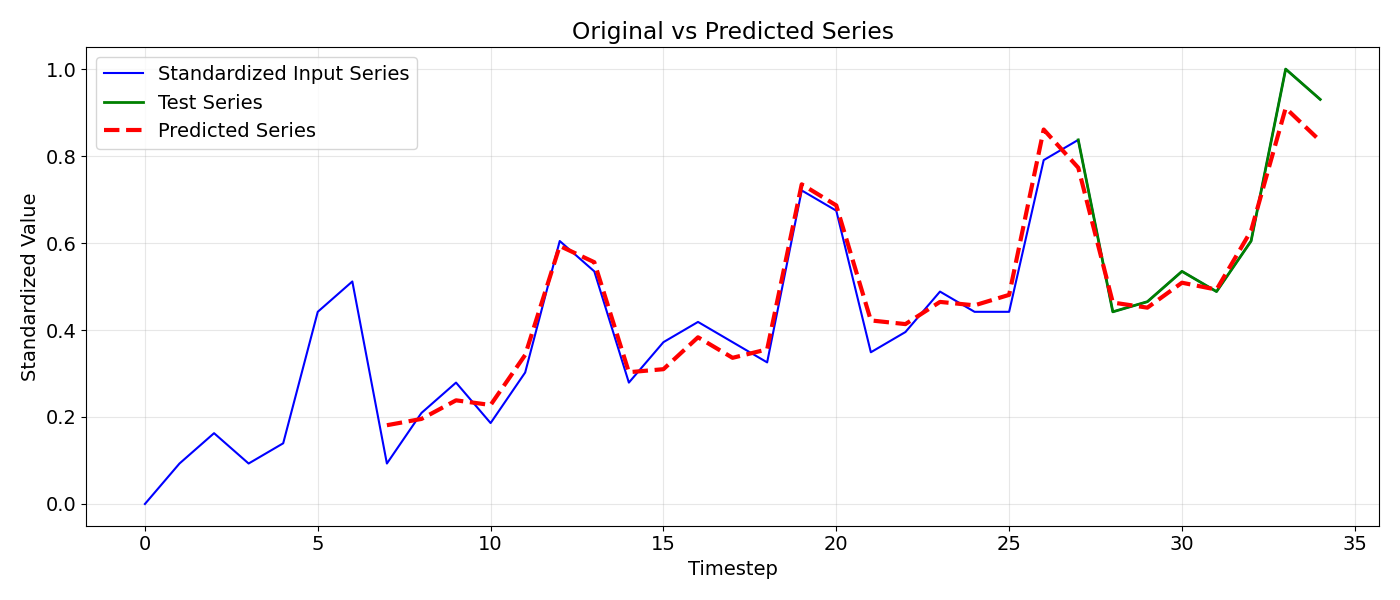
\includegraphics[width=1.0\linewidth]{restaurants.png}
    \caption{The Google trends restaurants dataseries}
    \label{fig:restaurants}
\end{figure}

Despite the limited data and restrictive configuration, the transformer is highly effective in modelling the input series, though its forecasting abilities are, as would be expected, less accurate. More significant tests are reported in Section \ref{sec:results}.

%%%%%%%%%%%%%%%%%%%%%%%%%%%%%%%%%%%%%%%%%%
\section{Computational results} \label{sec:results}

This section presents results obtained using our minimalist transformer architecture in forecasting well-known univariate benchmark data series.

First, we showcase the successive processing stages on the archetypal airline passenger data series \citep{BJ70}. Then, we present illustrative quantitative results on standard forecasting benchmark instances. \textcolor{blue}{Unless otherwise specified, the hyperparameters were optimized by means of the Optuna package \cite{ASY19}}.

\subsection{The airline passengers test case} \label{subsec:airlines}

The Airline Passengers time series is one of the most famous and widely used in data analysis and forecasting. It consists of 144 observations of the monthly total number of international airline passengers in thousands between 1949 and 1960. As it is a real-world case that is very easy to model and predict (it is known to be an ARMA(1,1)), it is commonly used as a first validation for new forecasting approaches.

When the model is applied to this series, setting aside the last 12 values for validation and accounting for the obvious 12-month seasonality, the successive encoding steps through the positional embedding - multi-head attention - layer norm pipeline produce the results shown in Figure \ref{fig:airlines}.

The series was preprocessed only by a standard min-max normalization, then it was projected into embeddings of size $m = 12$. Employing only $n = 12$ timesteps at a time, $118$ matrices $X \in \mathbb{R}^{12 \times 12}$ are obtained. Matrix $P$ used for positional embedding has the same dimensionality.

Next comes multi-head attention. We used 2 heads, and for each head we set $d_k = d_v = \frac{12}{2} = 6$. Therefore all matrices $W^h_Q$, $W^h_K$ and $W^h_V$ had dimensions $12 \times 6$. These provide the bases for computing the attention function, where each $h-th$ head gives rise to the matrix $A^h=\frac{Q_hK'_h}{d_h} \in \mathbb{R}^{n \times n}$, in our case $A^h \in \mathbb{R}^{12 \times 12}$. The successive {\em softmax} function does not change its dimensionality. After multiplying by $V_h$ we obtain the output of each head, of dimension $12 \times 6$. All outputs are then concatenated by row, giving rise to a matrix $A \in \mathbb{R}^{12 \times 12}$. The input dimension is then kept, when the output attention matrix is multiplied by matrix $W_O \in \mathbb{R}^{hd_v \times m}$ - in our case, of dimension $12 \times 12$. In summary, the values used for the parameters were: $n$=12, $m$=12, $k$=2,  $d_k$=$d_v$=6, $p$=48. The number of epochs set for learning was 400, the total number of parameters to learn in the transformer model resulted to be 5413.

\begin{figure}
	\centering
	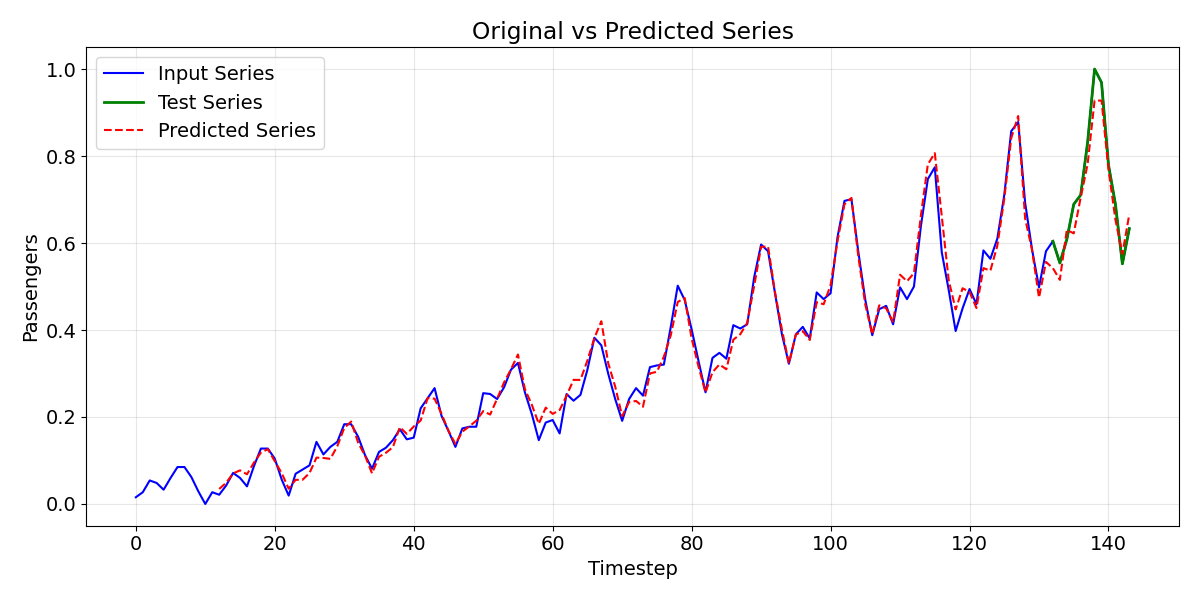
\includegraphics[width=1.0\linewidth]{airlines.png}
	\caption{The predictions of the model on the full airline series, comprising 132 training data-points and 12 evaluation points.}
	\label{fig:airlines}
\end{figure}

%%%%%%%%%%%%%%%%%%%%%%%%%%%%%%%%%%%%%%%%%%
\subsection{Benchmark results} \label{subsec:benchmark}

Our work aimed to provide a basic, simple architecture that could be used to fully understand the internal functioning and possibly form the basis for improvements, rather than a best-of-class architecture. However, it is important to validate its effectiveness in order to determine how representative it is of the possibilities offered by the transformer approach to data series forecasting. To this end, we ran both our system and a standard random forest forecaster, the RandomForestRegressor from scikit-learn \cite{GEW06}, on a standard forecasting benchmark.

The benchmark consisted of the monthly series from the M3 forecasting competition \cite{MH00}. The M3 dataset comprises a variety of time series from different domains and frequencies, including yearly, quarterly, monthly and other intervals. \textcolor{blue}{It contains the kind of seasonal and noisy data commonly encountered in business forecasting}. The monthly data subset includes 1428 real world time series collected at monthly intervals covering a wide range of domains, classified as:

\begin{itemize}
	\item {\it Macroeconomics} (e.g., unemployment rates, inflation, industrial production),
	\item {\it Microeconomics} (e.g., sales, orders, inventory levels for individual companies),
	\item {\it Industry} (e.g., combined production, sales, or demand in a broader industrial sector, not just a single firm)
	\item {\it Finance} (e.g., stock prices, exchange rates, interest rates),
	\item {\it Demographics} (e.g., population statistics, birth/death rates),
	\item {\it Others}, i.e., diverse, real-world time series that don’t belong to traditional economic or financial domains (e.g., energy consumption, transportation data)
\end{itemize}

The length of the monthly series varies, typically ranging from 48 to 126 observations (i.e., 4 to over 10 years of data) and for each series, participants were asked to forecast the next 18 months. This same forecast horizon has been used in our tests, and the following argument values: $n$=24, $m$=36, $k$=4, $d_k$=$d_v$=12, $p$=144. The number of epochs set for network learning was 400, the total number of parameters to learn in the transformer model resulted to be 46'189.

We ran each model on all the benchmark series, computing the RMSE on both the training and test sets. To determine whether the difference in forecast effectiveness was significant, a Mann–Whitney U-test has been conducted on the RMSE results for each aggregate separately. Table \ref{tab:aggregate} shows the results of the comparison aggregated over the type feature. The columns show:

\begin{itemize}
	\item {\it type}: type of the aggregate,
	\item {\it num}: number of series in the aggregate,
	\item {\it len}: average length of the series of the aggregate,
	\item {\it train}: number of series where the transformer had a lower RMSE on the training set,
	\item {\it test}: number of series where the transformer had a lower RMSE on the number of series where the transformer had a lower RMSE on the training set,
	\item {\it perc}: percentage of aggregate series where the transformer had a lower RMSE on the training set
	\item {\it pval}: p value of the Mann-Whitney U test.
\end{itemize}

\begin{table}[H]
\caption{Minimalist transformer and random forest, aggregate results}
\label{tab:aggregate}
\centering
%% \tablesize{} %% You can specify the fontsize here, e.g., \tablesize{\footnotesize}. If commented out \small will be used.
\begin{tabular}{ccccccc}
\toprule
{\bf type} & {\bf num} & len & {\bf train} & {\bf test} & {\bf perc} & {\bf pval}\\
\midrule
MICRO 		& 474 &  92.65 & 6 & 134 & 28.27 & 0.000\\
INDUSTRY 	& 334 & 140.02 & 3 & 123 & 36.83 & 0.042\\
MACRO 		& 312 & 130.88 & 3 & 101 & 32.37 & 0.021\\
FINANCE 	   & 145 & 124.40 & 1 &  68 & 46.90 & 0.247\\
DEMOGRAPHIC & 111 & 123.33 & 3 &  33 & 29.73 & 0.021\\
OTHER 		&  52 &  82.98 & 0 &  29 & 55.77 & 0.661\\
\bottomrule
\end{tabular}
\end{table}

The results in Table \ref{tab:aggregate}  show that, despite being outperformed as a modeller of the known part of the series, the transformer solution can already be competitive in forecasting, despite the limiting operational restrictions. The quality of the forecast depends on the structure of the data, resulting from dependency on the application domain. In the MICRO and DEMOGRAPHIC domains, transformers performed better than Random Forest in less than one-third of cases, whereas in FINANCE it was almost one-half, and in the OTHER domain even more than half the time. There is no statistical difference in performance between the two approaches for these last two domains, while Random Forest has a significantly lower average RMSE for the other four. \textcolor{blue}{The results of the tests are highly dependent on sample size. It is not surprising that the greatest indifference is observed for the least numerous sample. However, no aggregate has a sample size that renders the test irrelevant.}

\textcolor{blue}{As the M3 benchmark has been studied in depth, we can tentatively interpret these observations. Financial data is characterised by high volatility and weak or non-existent trends or seasonality. They therefore have a higher noise component, which appears to be better handled by transformers. In contrast, industry and macro data have stronger deterministic components, such as trends and seasonality (due to business cycles, yearly production seasonality, etc.), which are better captured by a decision tree-based model.
Seasonality is in fact much more pronounced in industry and demographics series, while finance has very weak seasonality and is often dominated by idiosyncratic shocks. A similar situation applies to trends in the series, where demographic and macroeconomic series exhibit clear long-term growth or decline. Finally, and most significantly, financial and 'other' series are subject to frequent regime shifts, whereas industry and macroeconomic series undergo structural breaks less frequently and exhibit more persistent regimes.}

\begin{table}[H]
\caption{Minimalist transformer and random forest, aggregate results, scaled data}
\label{tab:bestworse}
\centering
%% \tablesize{} %% You can specify the fontsize here, e.g., \tablesize{\footnotesize}. If commented out \small will be used.
\begin{tabular}{cccccccccc}
\toprule
id   & type        & trtrain & trtest & rftrain & rftest & $\Delta$train & $\Delta$test & trtime & rftime \\
\midrule
\small N1652 & \footnotesize MICRO       & 0.061 & 0.262 & 0.062 & 0.335 & -0.001 &-0.072& 0.07&0.15\\
\small N1546 & \footnotesize MICRO       & 0.168 & 0.526 & 0.068 & 0.306 & 0.1   &  0.219& 0.04&0.14\\
\small N1894 & \footnotesize INDUSTRY    & 0.133 & 0.290 & 0.058 & 0.433 & 0.074 & -0.142&0.11&0.22\\
\small N2047 & \footnotesize INDUSTRY    & 0.144 & 0.667 & 0.056 & 0.428 & 0.088 &  0.238&0.12&0.21\\
\small N2255 & \footnotesize MACRO       & 0.068 & 0.088 & 0.021 & 0.494 & 0.046 & -0.406&0.13&0.20\\
\small N2492 & \footnotesize MACRO       & 0.130 & 0.626 & 0.054 & 0.249 & 0.076 &  0.377&0.18&0.21\\
\small N2594 & \footnotesize FINANCE     & 0.074 & 0.597 & 0.015 & 0.737 & 0.059 & -0.140&0.13&0.19\\
\small N2658 & \footnotesize FINANCE     & 0.126 & 0.656 & 0.046 & 0.435 & 0.080 &  0.220&0.03&0.13\\
\small N2737 & \footnotesize DEMOGRAPHIC & 0.074 & 0.129 & 0.046 & 0.209 & 0.028 & -0.079&0.32&0.21\\
\small N2758 & \footnotesize DEMOGRAPHIC & 0.214 & 1.007 & 0.034 & 0.310 & 0.180 &  0.696&0.05&0.13\\
\small N2817 & \footnotesize OTHER       & 0.079 & 0.125 & 0.036 & 0.441 & 0.043 & -0.315&0.06&0.13\\
\small N2823 & \footnotesize OTHER       & 0.116 & 0.166 & 0.066 & 0.081 & 0.050 &  0.085&0.11&0.13\\
\bottomrule
\end{tabular}
\end{table}

Table \ref{tab:bestworse} shows details of the instances in each category for which transformers achieved the best and worst test results compared to random forest. The columns of the table contain data that refer to scaled series and are:
\begin{itemize}
	\item {\it id}: the id of the data series in the M3 collection;
	\item {\it type}: the category of the data series;
	\item {\it trtrain}: the absolute RMSE of the transformers model on the training part;
	\item {\it trtest}: the absolute RMSE of the transformers model on the test part, i.e., on the last 18 data points;
	\item {\it rftrain}: the absolute RMSE of the random forest model on the training part;
	\item {\it rftest}: the absolute RMSE of the random forest model on the test part, i.e., on the last 18 data points;
	\item {\it $\Delta$train}: the RMSE difference between transformers and random forest on the training part;
	\item {\it $\Delta$test}: the RMSE difference between transformers and random forest on the test part;
	\item {\it trtime}: the average time in seconds needed to train for a single epoch the Transformer on the respective series;
	\item {\it rftime}: the time in seconds needed to fit the random forest model on the training set.
\end{itemize}

The results in the table confirm that the RMSE values are comparable in all cases and that there are never differences in the order of magnitude, with values remaining relatively low when even considering that they were computed on max-min scaled series. In all categories, the transformers achieved a lower RMSE in at least one series. Figures \ref{fig:trbest} and \ref{fig:trworse} show plots of the actual series and the forecasts of the transformers and the random forest in cases where the transformers performed better and worse than the random forest, respectively.

\begin{figure}
	\centering
	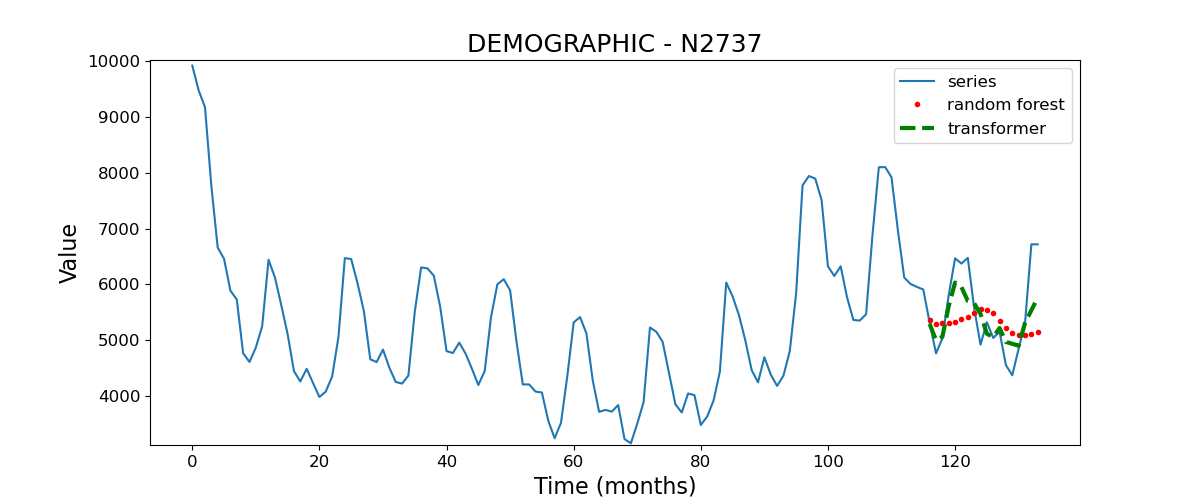
\includegraphics[width=1.0\linewidth]{N2737.png}
	\caption{Actual data, transformers and random forest forecast on series N2737.}
	\label{fig:trbest}
\end{figure}
\begin{figure}
	\centering
	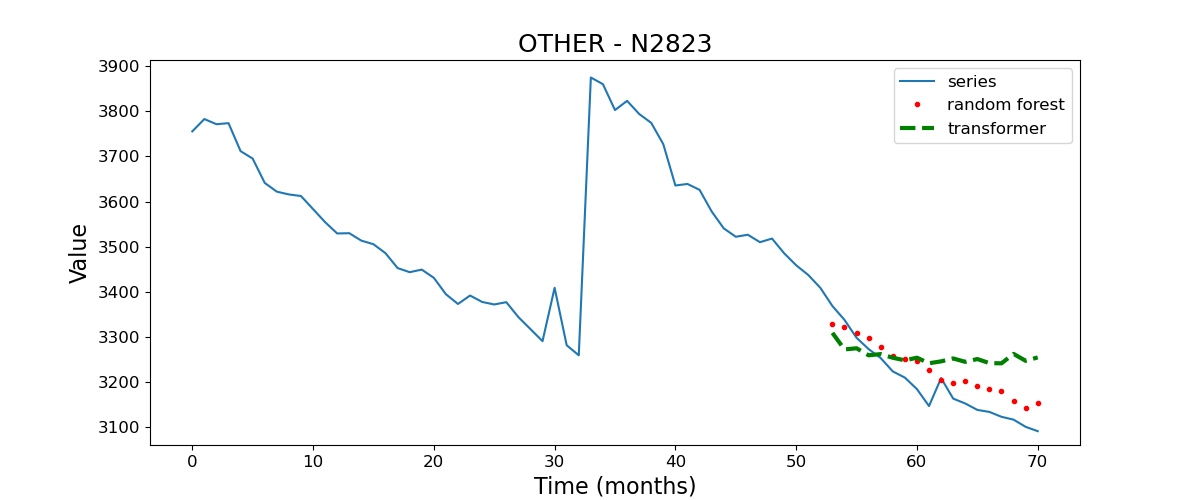
\includegraphics[width=1.0\linewidth]{N2823.png}
	\caption{Actual data, transformers and random forest forecast on series N2833.}
	\label{fig:trworse}
\end{figure}


\textcolor{blue}{To evaluate the scalability of the attention mechanism in capturing patterns, we conducted experiments on four longer time series. Table \ref{tab:long} below reports the information about the time series themselves and of the experiments' results. Each run had $24$ timesteps as input and had to predict $18$ points in time; each dataset, instead, had $870$ samples in the training set and $187$ in the test set. Some plot examples from the start of each series can be seen in Figure \ref{fig:long}.}

\begin{table}[H]
	\caption{Minimalist Transformer results over longer time series.}
	\label{tab:long}
	\centering
	\begin{tabular}{l cccccccc}
		\toprule
		name & trtrain & trtest & rftrain & rftest & $\Delta$train & $\Delta$test & trtime & rftime  \\
		\midrule
		\small SDI\_Temp\_1m 			& 0.047 & 0.143 & 0.012 & 0.170 & 0.035 & -0.027 & 5.06 & 2.52  \\
 	\small 	Vapor\_Pressure\_Avg\_2		&  0.114 & 0.167 & 0.038 & 0.170 & 0.076 & -0.003 & 4.93 & 10.99 \\
 	\small 	WS\_ms\_Avg 				& 0.175 & 0.190 & 0.061 & 0.191 & 0.114 & -0.001 & 4.96 & 19.28 \\
 	\small 	WTemp\_C1\_Avg 				& 0.047 & 0.157 & 0.011 & 0.195 & 0.036 & -0.038 & 4.93 & 12.73 \\
		\bottomrule
	\end{tabular}
\end{table}

\begin{figure}
	\centering
	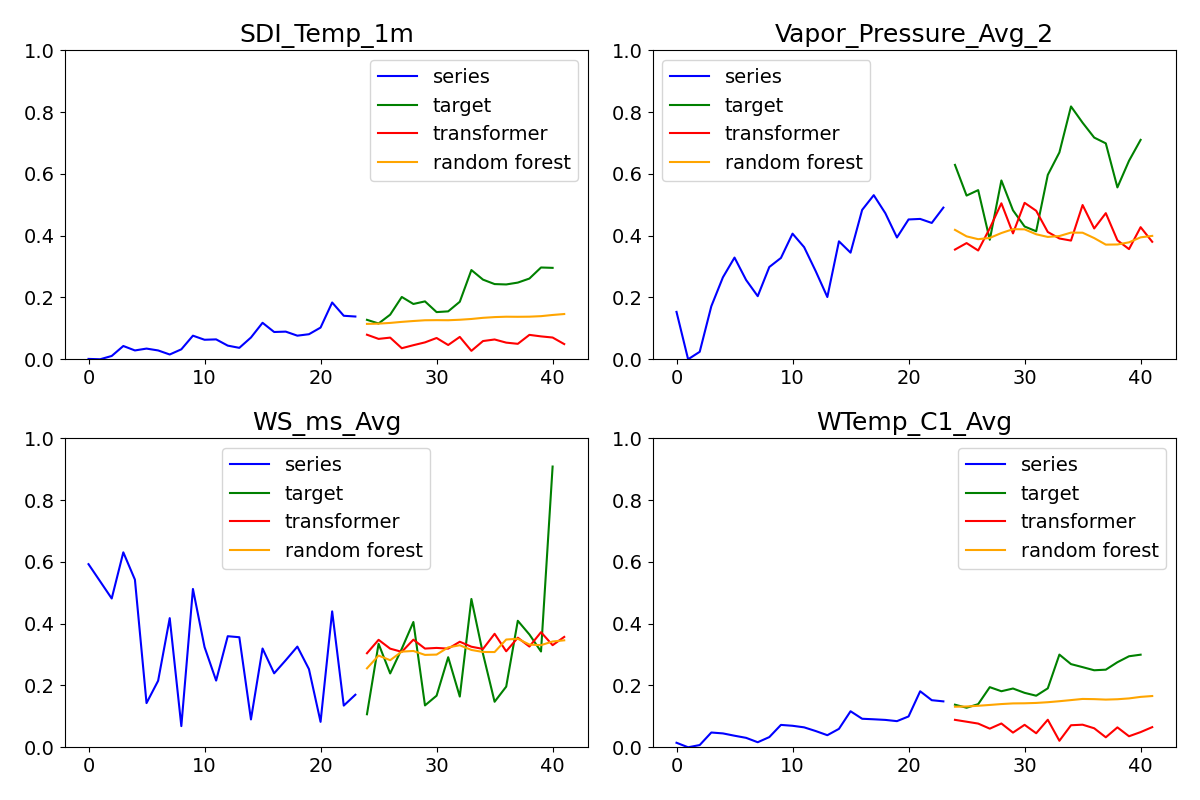
\includegraphics[width=1.0\linewidth]{long.png}
	\caption{The series and the respective predictions of the Minimalistic Transformer model along with the Random Forest regressor.}
	\label{fig:long}
\end{figure}

\textcolor{blue}{Other comparisons have been performed against other models, complementing the Random Forest baseline and offering a broader perspective by including recent transformer-based approaches. These comprise the Chronos model \cite{chronos}, TCAN (Temporal Convolution Attention Network) \cite{tcan}, ARIMA and ETS. The autoregressive models relied on their statsmodels implementation \cite{SP10} using pmdarima's stepwise approach for hyperparameter tuning \cite{S17}. The RMSE test results are shown for the series listed in Table \ref{tab:comparisons}}.
\begin{table}[H]
	\caption{Minimalist transformer compared to other baseline models.}
	\label{tab:comparisons}
	\centering
	\begin{tabular}{c|ccccc}
		\toprule
		id   & trtest & chronos & tcan & arima & ets \\
		\midrule
		N1652 & 0.262 & 0.5238 & 0.0745 & 0.1199 & 0.1203 \\
		N1546 & 0.526 & 0.4107 & 0.1700 & 0.2382 & 0.2348 \\
		N1894 & 0.290 & 0.3803 & 0.2504 & 0.4085 & 0.3640 \\
		N2047 & 0.667 & 0.4639 & 0.2547 & 0.1332 & 0.1509 \\
		N2255 & 0.088 & 0.4095 & 0.1064 & 0.2011 & 0.0330 \\
		N2492 & 0.626 & 0.3174 & 0.2204 & 0.2844 & 0.2237 \\
		N2594 & 0.597 & 0.3647 & 0.1155 & 0.0138 & 0.0478 \\
		N2658 & 0.656 & 0.3626 & 0.1913 & 0.2489 & 0.3690 \\
		N2737 & 0.129 & 0.2117 & 0.1176 & 0.2381 & 0.3063 \\
		N2758 & 1.007 & 0.4105 & 0.3582 & 0.2126 & 0.1939 \\
		N2817 & 0.125 & 0.5384 & 0.1580 & 0.1436 & 0.1263 \\
		N2823 & 0.166 & 0.4495 & 0.3048 & 0.3025 & 0.3257 \\
		\bottomrule
	\end{tabular}
\end{table}

\subsection{Ablation Studies}

In Table \ref{tab:ablation} it's possible to see the effects of removing or editing computational blocks of the Encoder, as drawn in Figure \ref{fig:enc}, on the performance of the entire model. Each cell reports respectively the training and the testing loss of the configuration in the column of the instance in the row, and the corresponding loss, while the columns show:

\begin{itemize}
	\item {id}: the id of the data series in the M3 collection;
	\item {1-sized embeddings}: results using embeddings of a single value (i.e., no embedding), lines \ref{enc:seca1}-\ref{enc:seca2} of Algorithm \ref{algo:encoding};
	\item {No PE}: results without positional encoding, line \ref{enc:positional} of Algorithm \ref{algo:encoding};
	\item {Single Head}: results with single head instead than mutihead attention, lines \ref{enc:multihead1}-\ref{enc:multihead2} of Algorithm \ref{algo:encoding}; 
	\item {No Add\&Norm 1}: results removing the first Add \& Norm block, line \ref{enc:addnorm1} of Algorithm \ref{algo:encoding};
	\item {No FF}: results removing the feedforward network, line \ref{enc:ffn} of Algorithm \ref{algo:encoding};
	\item {No Add\&Norm 2}: results removing the second Add \& Norm block, line \ref{enc:addnorm2} of Algorithm \ref{algo:encoding};
	\item {Baseline}: results of the complete model.
\end{itemize}
\end{itemize}

As the model is quite small, comprising just a single encoder block and a single decoder block, the overall effect is visible but not particularly impactful. As expected, the baseline model achieves the best loss value over the validation data, while the model without the feedforward network is still almost equivalent to it, removing any other component has comparable highly disruptive effect. Furthermore, the full model has the fourth highest training loss value. This, alongside the validation result, indicates the model's ability to generalize over the training data.

As the model is quite small, comprising just a single encoder block and a single decoder block, the overall effect is visible but not particularly impactful. As expected, the baseline model achieves the best loss value over the validation data. Moreover, it has the fourth highest training loss value, which, alongside the validation result, indicates the model's ability to generalize over the training data.

\begin{sidewaystable}
	\caption{Ablation studies.}
	\label{tab:ablation}
\begin{table}[H]
	\centering
	\begin{tabular}{|c | ccccccc | c}
		\toprule
		id & Single Head & No FF & No Add\&Norm 1 & No Add\&Norm 2 & 1-sized embeddings & No PE &  \iffalse No Output &\fi Baseline \\
		\midrule
		N1652 & 0.175/0.327 & 0.188/0.329 & 0.183/0.332 & 0.180/0.327 & 0.410/0.568 & 0.183/0.301 &\iffalse 0.183/0.323 &\fi 0.179/0.337  \\
		N1546 & 0.194/0.353 & 0.185/0.290 & 0.211/0.480 & 0.190/0.330 & 0.605/0.319 & 0.190/0.301 &\iffalse 0.195/0.407 &\fi 0.197/0.354  \\
		N1894 & 0.142/0.496 & 0.188/0.385 & 0.132/0.325 & 0.156/0.524 & 0.243/0.370 & 0.108/0.512 &\iffalse 0.149/0.260 &\fi 0.152/0.211  \\
		N2047 & 0.161/0.252 & 0.157/0.448 & 0.168/0.255 & 0.134/0.432 & 0.181/0.253 & 0.099/0.488 &\iffalse 0.141/0.324 &\fi 0.173/0.344  \\
		N2255 & 0.117/0.619 & 0.126/0.587 & 0.124/0.603 & 0.121/0.608 & 0.775/0.208 & 0.068/0.596 &\iffalse 0.097/0.566 &\fi 0.119/0.577  \\
		N2492 & 0.157/0.438 & 0.113/0.272 & 0.154/0.571 & 0.143/0.598 & 0.267/0.340 & 0.097/0.559 &\iffalse 0.133/0.380 &\fi 0.114/0.167  \\
		N2594 & 0.133/0.728 & 0.125/0.800 & 0.115/0.640 & 0.154/0.656 & 0.542/0.121 & 0.082/0.615 &\iffalse 0.118/0.523 &\fi 0.137/0.653  \\
		N2658 & 0.143/0.547 & 0.210/0.268 & 0.182/0.313 & 0.184/0.418 & 0.215/0.246 & 0.166/0.428 &\iffalse 0.190/0.234 &\fi 0.186/0.380  \\
		N2737 & 0.164/0.226 & 0.137/0.245 & 0.131/0.316 & 0.116/0.255 & 0.168/0.198 & 0.099/0.199 &\iffalse 0.160/0.215 &\fi 0.154/0.193  \\
		N2758 & 0.238/0.392 & 0.273/0.335 & 0.276/0.401 & 0.253/0.479 & 0.371/0.221 & 0.091/0.711 &\iffalse 0.272/0.366 &\fi 0.229/0.357  \\
		N2817 & 0.267/0.422 & 0.254/0.414 & 0.262/0.428 & 0.240/0.294 & 0.588/0.200 & 0.167/0.466 &\iffalse 0.226/0.386 &\fi 0.268/0.341  \\
		N2823 & 0.300/0.200 & 0.307/0.221 & 0.308/0.347 & 0.293/0.178 & 3.025/2.723 & 0.233/0.177 &\iffalse 0.286/0.218 &\fi 0.308/0.220  \\
		\midrule
		 avg. & 0.183/0.417 & 0.189/0.383 & 0.187/0.418 & 0.180/0.425 & 0.616/0.481 & 0.132/0.446 &\iffalse 0.179/0.350 &\fi 0.185/0.345  \\
		\bottomrule
	\end{tabular}
\end{table}
\end{sidewaystable}

\subsection{Interpretability}
As an additional view, Figure \ref{fig:attention} shows - for the restaurant Google Trends series - the contribution of each timestep that the Decoder gives to both the encoded input time series and to the autoregressively generated output timestep. The bigger the circle around a certain timestep, the greater the attention weight given by the trained model for inference.

More specifically, the attention of the input series - in blue - is extracted by the weights of the Cross-Attention layer, while the attention contribution of the generated series - in green - is examined in the Self-Attention layer.

The results are aligned with what one might expect the model to learn about a seasonal trajectory. For instance, it can be seen that for the generation of the first timestep (titled in Figure \ref{fig:attention} as "Step 1") the model depends on the timestep seven days prior - which is when a certain seasonal small rise happens. A similar argument could be given by noticing that - from the generation of the fifth step onwards - the model heavily uses the peak value of the input series, probably to extract information about the correct value of the new seasonal peak.

Another interesting observation that emerges from the above example is that the model tries to focus on specific timesteps, almost ignoring entirely other. Since the difference between the those timesteps is small, the model tries best to gather as much information as possible from a few significant timesteps, rather than relying on too many similar ones.

\begin{figure}
	\centering
	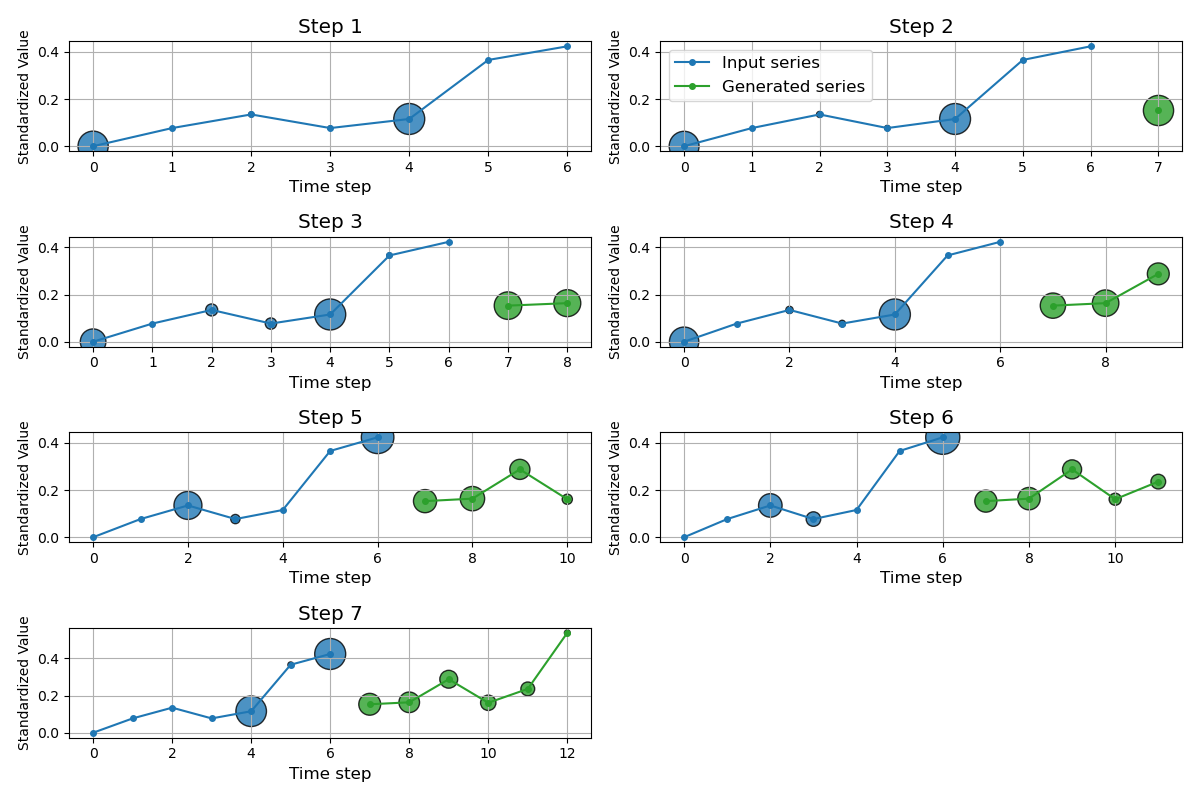
\includegraphics[width=1.0\linewidth]{attention.png}
	\caption{The contribution of each timestep for each generated output value.}
	\label{fig:attention}
\end{figure}

%%%%%%%%%%%%%%%%%%%%%%%%%%%%%%%%%%%%%%%%%%
\section{Conclusions} \label{sec:conclusions}

\textcolor{blue}{This work presents a minimalist transformer architecture that is specifically designed for univariate time series forecasting}. Rather than proposing yet another cutting-edge variant, our contribution lies in systematically reducing the architecture to its essential components and documenting all relevant steps of the encoder, decoder and learning procedures in pseudocode. Our aim was to provide a transparent and replicable baseline for researchers and practitioners interested in understanding the core mechanisms of transformers when applied to forecasting tasks.

\textcolor{blue}{The model is evaluated using a set of standard forecasting benchmarks and compared its performance with that of a random forest forecaster}. Although the minimalist transformer does not outperform the most sophisticated state-of-the-art models, it consistently achieves comparable accuracy, particularly for time series with long-term dependencies, where attention mechanisms can exploit global context more effectively than purely tree-based methods.

\textcolor{blue}{Beyond raw predictive performance, our findings highlight two key outcomes: clarity and accessibility. By explicitly exposing each functional step, our framework lowers the barrier for newcomers to the transformer literature and the field of time series forecasting}.

The robustness of the transformer paradigm is also evident, as even a stripped-down version of the model demonstrates stable forecasting ability. This suggests that many performance gains in advanced variants stem from relatively minor architectural refinements.

\textcolor{blue}{Although designed for univariate forecasting, the proposed architecture can be readily extended to the multivariate case by adapting the input encoding to jointly represent the target variable and external predictors, thereby enabling the model to explicitly learn and exploit correlations between them}.

\textcolor{blue}{In a research landscape often dominated by increasingly complex architectures, our study highlights the importance of transparent baselines}. Future work may explore the impact of specific enhancements, such as seasonal embeddings, multi-head configurations or hybridization with statistical components, on forecasting performance when added to this minimalist core.

%%%%%%%%%%%%%%%%%%%%%%%%%%%%%%%%%%%%%%%%%%
%% Optional
\appendixtitles{no} % Leave argument "no" if all appendix headings stay EMPTY (then no dot is printed after "Appendix A"). If the appendix sections contain a heading then change the argument to "yes".
\appendixstart
\appendix
\section[\appendixname~\thesection]{} \label{sec:appendix}
%\subsection[\appendixname~\thesubsection]{}
This appendix contains all values of the trained matrices obtained for the encoding of the running example described in Section \ref{sec:transformer}.

\noindent Table ~\ref{tab:matX} shows the first embedded matrix, $X$, which encodes the input series. The matrix has been transposed for the sake of compact presentation.

\begin{table}[ht]
	\centering
	\caption{The first 7$\times$4 embedded matrix $X$ used in the encoding process.}
	\label{tab:matX}
	$
	X^T =	\begin{bmatrix}
-0.4499 & -0.3722 & -0.3139 & -0.3722 & -0.3333 & -0.0808 & -0.0225 \\
 0.3955 &  0.1987 &  0.0512 &  0.1987 &  0.1004 & -0.5389 & -0.6865 \\
 0.0499 &  0.2140 &  0.3371 &  0.2140 &  0.2961 &  0.8295 &  0.9526 \\
-0.0958 & -0.0135 &  0.0483 & -0.0135 &  0.0277 &  0.2953 &  0.3570
\end{bmatrix}
	$
\end{table}

\begin{table}[ht]
	\centering
	\caption{The projection vectors used to convert each scalar timestep in an embedding, and viceversa.}
	\label{tab:seca}
	$
	W_i = 	\begin{bmatrix}
				0.8354 \\
				-2.1147 \\
				1.7644 \\
				0.8851
			\end{bmatrix} \;
	b_i = 	\begin{bmatrix}
				-0.4499 \\  0.3955 \\  0.0499 \\ -0.0958
			\end{bmatrix} \quad\;
	W_o = 	\begin{bmatrix}
				 0.3003 \\ -0.1796 \\  0.3854 \\  0.0305
			\end{bmatrix} \;
	b_o = 	\begin{bmatrix}
				0.0597
			\end{bmatrix}
	$
\end{table}

\noindent Table ~\ref{tab:matP} shows the positional encoding matrix, $P$. The matrix has been transposed for the sake of compact presentation.

\begin{table}[ht]
	\centering
	\caption{The 7$\times$4 positional encoding matrix $P$.}
	\label{tab:matP}
	$
	P^T = \begin{bmatrix}
	0.2843 & -0.8508 & -0.7088 & -1.1406 &  1.0270 &  0.9304 &  0.4463 \\
	1.0329 & -0.4291 &  0.0881 & -0.1644 & -0.6551 &  0.6012 & -0.3370 \\
	0.8908 & -0.2810 &  0.8743 &  0.5641 & -1.0543 & -0.4678 &  1.4571 \\
	0.4260 &  0.2978 & -0.8110 & -0.1593 & -0.5840 & -1.0103 & -0.7960
	\end{bmatrix}
	$
\end{table}

\noindent Table \ref{tab:matWq} presents the query matrices $W^1_q$ and $W^2_q$, the key matrices $W^1_k$ and $W^2_k$ and the value matrices $W^1_v$ and $W^2_v$ for the two heads used in the restaurant running example.

\begin{table}[ht]
	\centering
	\caption{Query, key and value matrices.}
	\label{tab:matWq}
	
	\begin{tabular}{rlrl}  % two centered columns
		$W^1_q$= & 
		$
		\begin{bmatrix}
		0.1310 &  0.5068 &  0.2681 &  0.2951 \\
        0.3385 &  1.0323 & -0.0560 &  0.2226
		\end{bmatrix}
		$
		&
		$W^2_q$ =
		&
		$
		\begin{bmatrix}
		-0.8557 & 0.4819 & -0.5107 &  0.1844 \\
        0.4872 & -0.1906 &  0.6404 & -0.7132
		\end{bmatrix}
		$
%	\end{tabular}	
%\end{table}
%
%\begin{table}[ht]
%	\centering
%	\caption{Matrices $W^1_k$ and $W^2_k$}
%	\label{tab:matWk}
%	
%	\begin{tabular}{rlrl}  
\\
		$W^1_k$ = & 
		$
		\begin{bmatrix}
		-0.7092 & -0.1109 & -0.6519 & -0.1403 \\
        -0.4628 & -0.4405 &  0.3128 &  0.2569
		\end{bmatrix}
		$
		&
		$W^2_k$= &
		$
		\begin{bmatrix}
		0.3696 & -0.8603 & -0.1482 &  1.2098 \\
        -0.2819 & 0.7551 & -0.4609 & -1.2695
		\end{bmatrix}
		$
%	\end{tabular}	
%\end{table}
%
%\begin{table}[ht]
%	\centering
%	\caption{Matrices $W^1_v$ and $W^2_v$}
%	\label{tab:matWv}
%	
%	\begin{tabular}{rlrl}  
\\
		$W^1_v$ = & 
		$
		\begin{bmatrix}
			0.2794 & -0.8501 & 0.0569 & -0.0530 \\
        -0.5428 &  0.9581 & -0.0329 & -0.2587
		\end{bmatrix}
		$
		&
		$W^2_v$ = &
		$
		\begin{bmatrix}
		0.0266 & -0.8855 &  0.0607 & -0.1688 \\
        -0.9599 & -0.0645 & -0.2187 & -0.3482
		\end{bmatrix}
		$
	\end{tabular}	
\end{table}

\begin{table}
	\centering
	\caption{The additive bias arrays learned for projection.}
	\label{tab:bias}
	\begin{tabular}{c c c c}
		$b^{Q}_1 = \begin{bmatrix} 0.6879 \\ 0.3649 \end{bmatrix}$ 
		& $b^{K}_1 = \begin{bmatrix} 0.1048 \\ -0.0416 \end{bmatrix}$ 
		& $b^{Q}_2 = \begin{bmatrix}-0.4185 \\ 0.8086 \end{bmatrix}$ 
		& $b^{K}_2 = \begin{bmatrix} -0.2673 \\  0.0098 \end{bmatrix}$ \\
		$b^{V}_1 = \begin{bmatrix} -0.1740 \\  0.0893 \end{bmatrix}$ 
		& $b^{O}_1 = \begin{bmatrix} -0.3292 \\  0.4357 \end{bmatrix}$ 
		& $b^{V}_2 = \begin{bmatrix} 0.0213 \\ -0.0516 \end{bmatrix}$ 
		& $b^{O}_2 = \begin{bmatrix} -0.2850 \\ -0.2149 \end{bmatrix}$ \\
	\end{tabular}
\end{table}

\noindent Table \ref{tab:matA} presents the attention matrix as resulting after the multihead attention phase for the restaurant time series.

\begin{table}[ht]
	\centering
	\caption{The matrix $A$ obtained.}
	\label{tab:matA}
	$
	A = 
\begin{bmatrix}
 0.0531 & -0.1152 & -0.0142 & -0.0760 & -0.0043 &  0.1103 &  0.1638 \\
 0.1000 &  0.2736 &  0.1393 &  0.2191 &  0.1116 &  0.0060 & -0.0616 \\
-0.4575 & -0.3464 & -0.4285 & -0.3830 & -0.4366 & -0.4860 & -0.4923 \\
 0.4941 &  0.1239 &  0.2288 &  0.1804 &  0.1319 &  0.2962 &  0.1124
\end{bmatrix}
	$
\end{table}

\noindent  Table \ref{tab:matWO} shows the matrix used to restore the needed dimensionality after the multihead attention computation.

\begin{table}[ht]
	\centering
	\caption{The matrix $W^O$ used for reprojection of the running example.}
	\label{tab:matWO}
	$
	W^O =   \begin{bmatrix}
				-0.1143 &  0.3255 &  0.1047 &  0.5301 \\
        0.1422 & -0.2276 &  0.0155 & -0.5644 \\
        0.1575 & -0.1060 &  0.1315 & -0.1953 \\
        0.3641 &  0.9191 & -0.2459 & -0.0482
			\end{bmatrix}
	$
\end{table}

\noindent Tables \ref{tab:matW1b1} and \ref{tab:matW2b2} show the weights learnt by the feed-forward neural network used at the end of the encoding phase. They show the weights of the hidden and output layers, respectively.

\begin{table}[ht]
	\centering
	\caption{Feedforward network, weights of the internal layer.}
	\label{tab:matW1b1}
	
	\begin{tabular}{rlrl}  
		$W_1^T$ = & 
		$
	\begin{bmatrix}
		0.3067 &  0.1809 &  0.0673 &  0.5560 \\
		-0.1806 & -0.0553 & -0.2755 &  0.2545 \\
		-0.1128 & -0.1211 & -0.4158 &  0.5880 \\
		-0.1154 &  0.1402 &  0.0267 &  0.5364 \\
		0.0962 & -0.6581 & -0.2307 &  1.0214 \\
		0.0897 & -0.2100 &  0.1455 &  0.3424 \\
		-0.4518 &  0.2141 & -0.9220 &  1.0428 \\
		-0.3704 &  0.0218 & -0.4648 &  0.0920 \\
		-0.1018 & -0.1424 & -0.3883 &  0.4627 \\
		-0.0223 &  0.2030 & -0.2052 &  0.6145 \\
		0.1926 & -0.8201 & -0.0567 &  0.3366 \\
		0.0048 & -0.0324 & -0.0757 &  0.3328 \\
		-0.2997 &  0.3305 & -0.5676 &  0.5782 \\
		0.0013 & -0.1013 & -0.1348 & -0.1666 \\
		0.0737 &  0.0930 &  0.0206 &  0.0936 \\
		-0.2211 & -0.2244 & -0.3285 & -0.1195
		\end{bmatrix}
			$
		&
		$b_1$ = &
		$
\begin{bmatrix}
	-0.3033 \\
	-0.4938 \\
	-0.3991 \\
	-0.7121 \\
	-0.7605 \\
	-0.4844 \\
	-0.7139 \\
	-0.4224 \\
	-0.4635 \\
	-0.7017 \\
	-0.4705 \\
	-0.2822 \\
	-0.3001 \\
	-0.3100 \\
	-0.2118 \\
	-0.3648
\end{bmatrix}
		$
	\end{tabular}	
\end{table}

\begin{table}[ht]
	\centering
	\caption{Feedforward network, weights of the output layer.}
	\label{tab:matW2b2}
	
	\begin{tabular}{rlrl}  
		$W_2$ = & 
		$
	\begin{bmatrix}
-0.0902 &  0.0623 & -0.0051 & -0.0214 \\
 0.2824 & -0.1389 &  0.1038 &  0.0440 \\
-0.1227 &  0.1329 & -0.0587 & -0.3040 \\
 0.2578 & -0.4245 &  0.7379 &  0.2276 \\
-0.1491 &  0.4089 & -0.2755 & -0.6134 \\
 0.0673 &  0.0081 & -0.1963 & -0.0560 \\
 0.3649 & -0.1506 & -0.5302 &  0.6227 \\
 0.0849 & -0.1017 & -0.0649 &  0.2134 \\
 0.2211 &  0.0406 &  0.0487 &  0.1118 \\
 0.0785 &  0.1100 & -0.1416 &  0.1657 \\
-0.0010 & -0.3243 & -0.2919 &  0.5994 \\
-0.1367 & -0.1310 &  0.1522 &  0.0323 \\
-0.2234 & -0.0427 & -0.1288 &  0.0573 \\
-0.0032 & -0.0585 & -0.0134 & -0.1194 \\
-0.1594 & -0.1936 & -0.1171 &  0.0181 \\
 0.0751 &  0.1026 &  0.1138 &  0.1537
\end{bmatrix}
		$
		&
		$b_2$ = &
		$
		\begin{bmatrix}
			0.0467 \\  0.0970 \\ -0.1583 \\ -0.2808
		\end{bmatrix}
		$
	\end{tabular}	
\end{table}


%\section[\appendixname~\thesection]{}
%All appendix sections must be cited in the main text. In the appendices, Figures, Tables, etc. should be labeled, starting with %``A''---e.g., Figure A1, Figure A2, etc.

%%%%%%%%%%%%%%%%%%%%%%%%%%%%%%%%%%%%%%%%%%
%% optional
%\supplementary{The following supporting information can be downloaded at:  \linksupplementary{s1}, Figure S1: title; Table S1: title; Video S1: title.}

% Only used for preprtints:
% \supplementary{The following supporting information can be downloaded at the website of this paper posted on \href{https://www.preprints.org/}{Preprints.org}.}

%%%%%%%%%%%%%%%%%%%%%%%%%%%%%%%%%%%%%%%%%%
% CRITICAL: Force all pending floats to be output HERE
\clearpage

\authorcontributions{All authors contributed equally to the work and have read and agreed to the published version of the manuscript.}

\funding{This research received no external funding}

\dataavailability{In this section, please provide details regarding where data supporting reported results can be found, including links to publicly archived datasets analyzed or generated during the study.Suggested Data Availability Statements are available in section ``MDPI Research Data Policies'' at \url{https://www.mdpi.com/ethics}.} 

\acknowledgments{No generative AI has been used for purposes such as generating text, data, or graphics, or for study design, data collection, analysis, or interpretation of data. AI-assisted tools were only used to check the spelling, syntax and style of the writing.}

\conflictsofinterest{The authors declare no conflicts of interest.} 


\abbreviations{Abbreviations}{
The following abbreviations are used in this manuscript:
\\

\noindent 
\begin{tabular}{@{}ll}
MDPI & Multidisciplinary Digital Publishing Institute\\
DOAJ & Directory of open access journals\\
TLA & Three letter acronym\\
LD & Linear dichroism
\end{tabular}
}

% References
\externalbibliography{yes}
%\bibliographystyle{mdpi}
\bibliography{bibliography}

%%%%%%%%%%%%%%%%%%%%%%%%%%%%%%%%%%%%%%%%%%
%\isPreprints{}{% This command is only used for ``preprints''.
%\begin{adjustwidth}{-\extralength}{0cm}
%} % If the paper is ``preprints'', please uncomment this parenthesis.
%\printendnotes[custom] % Un-comment to print a list of endnotes


% If authors have biography, please use the format below
%\section*{Short Biography of Authors}
%\bio
%{\raisebox{-0.35cm}{\includegraphics[width=3.5cm,height=5.3cm,clip,keepaspectratio]{Definitions/author1.pdf}}}
%{\textbf{Firstname Lastname} Biography of first author}
%
%\bio
%{\raisebox{-0.35cm}{\includegraphics[width=3.5cm,height=5.3cm,clip,keepaspectratio]{Definitions/author2.jpg}}}
%{\textbf{Firstname Lastname} Biography of second author}

%%%%%%%%%%%%%%%%%%%%%%%%%%%%%%%%%%%%%%%%%%
%% for journal Sci
%\reviewreports{\\
%Reviewer 1 comments and authors’ response\\
%Reviewer 2 comments and authors’ response\\
%Reviewer 3 comments and authors’ response
%}
%%%%%%%%%%%%%%%%%%%%%%%%%%%%%%%%%%%%%%%%%%
\PublishersNote{}
%\isPreprints{}{% This command is only used for ``preprints''.
%\end{adjustwidth}
%} % If the paper is ``preprints'', please uncomment this parenthesis.
\end{document}

